\documentclass[conference]{IEEEtran}
\include{psfig}
\include{epsfig}
\usepackage{algorithm}
\usepackage{algorithmic}
\usepackage{rotating}
\usepackage{fontenc}
\usepackage{graphicx}
\usepackage{amsfonts}
\usepackage{amsmath}
\usepackage{cite}
\usepackage{proba}
\usepackage{amssymb,latexsym}
\usepackage{subfigure}
\usepackage{graphicx}
\usepackage{dsfont,multirow}
\usepackage{float}
%\interdisplaylinepenalty=2500

\newcommand{\be}{\begin{equation}}
\newcommand{\ee}{\end{equation}}
\newcommand{\bd}{\begin{displaymath}}
\newcommand{\ed}{\end{displaymath}}
\newcommand{\bear}{\begin{IEEeqnarray}}
\newcommand{\eear}{\end{IEEEeqnarray}}
\newcommand{\bo}[1]{\textbf{\emph{#1}}}


\newtheorem{lem}{Lemma}
\newtheorem{defn}{Definition}
\newtheorem{prop}{Property}
\newtheorem{prosi}{Proposition}
\newtheorem{thm}{Theorem}
\newtheorem{exmp}{Example}
%\usepackage{tikz}
%\usetikzlibrary{backgrounds}	% drawing the background after the %foreground
%\usetikzlibrary{shapes.geometric}
%\usepackage{enumitem}
%\let\labelindent\relax
%\newcommand{\keywords}[1]{\par\addvspace\baselineskip
%\noindent\keywordname\enspace\ignorespaces#1}


\def\proof{\noindent\hspace{2em}{\itshape Proof: }}


%\usepackage{here}

% LLNCS model

\begin{document}
\title{Mathematical methods for performance analysis of hysteresis queues}
%\thanks{partially supported by French research project ANR-MARMOTE}

%\numberofauthors{4}

\author{
\IEEEauthorblockN{M. Kandi} 
\and
\IEEEauthorblockN{F. {A\"{\i}t Salaht}}  
\and
\IEEEauthorblockN{H. Castel-Taleb}
\IEEEauthorblockA{INSTITUT TELECOM/Telecom SudParis\\
SAMOVAR, UMR 5157\\
9, rue Charles Fourier, 91011 Evry Cedex, France \\
Email: hind.castel@it-sudparis.eu}
\and
\IEEEauthorblockN{E. Hyon}
\IEEEauthorblockA{Sorbonne Universit{\'e}s, \\
UPMC Univ Paris 06,\\ 
CNRS, LIP6 Paris UMR 7606, \\
4 place Jussieu 75005 Paris}
\IEEEauthorblockA{Universit{\'e} Paris Nanterre}
}

%\institute{
%INSTITUT TELECOM,
%Telecom SudParis \\
% 9, rue Charles Fourier
%91011 Evry Cedex, France\\
%\{farah.ait-salaht, hind.castel,\}@it-sudparis.eu   }

%\author{\IEEEauthorblockN{Farah A\"{\i}t-Salaht, Hind Castel \\}
%\IEEEauthorblockA{INSTITUT TELECOM/Telecom SudParis\\
%SAMOVAR, UMR 5157\\
%9, rue Charles Fourier, 91011 Evry Cedex, France \\
%Email: \{farah.ait\_salaht, hind.castel\}@it-sudparis.eu}}


\maketitle


\begin{abstract}
Considering a cloud system, we propose in this paper to evaluate the performance of a data center using mathematical methods. Modeled as a hysteresis 
queueing system, a data center is characterized by a forward and backward threshold which allow to represent its dynamic behavior.
The client requests (or jobs) are represented by a Poisson process which arrive into the buffers and are executed by Virtual Machines (VMs). 
According to the occupation of  the queue and the thresholds, the VMs are activated  and deactivated by block. The system is represented by a complex 
Markov chain which  is difficult to analyze when the size of the system is huge. We propose to use in this case different mathematical methods in 
order to compute the steady-state probability distribution. We propose to apply  the SCA (Stochastic Complement Analysis) method in order to aggregate 
the state space. Another method which we develop is based on the numerical analysis of the system, it is the QBD (Quasi Birth and Death method).  
We propose also to use the balance equations in order to derive exact formulas for the steady-state probability distribution.
We present some numerical results for the performance measures in order to compare the  methods from their accuracy and the computation times.
\end{abstract}


\section{Introduction}

One of the most significant recent progresses in the field of information and communication technology is Cloud computing, which may
change the way people do computing and manage information. In this environment, a pool of abstracted, virtualized, dynamically-scalable
computing functions and services   are made accessible over the internet to remote users in an on-demand fashion, without the need for  
infrastructure investments and maintenance.

Virtualization plays a key role in the success of cloud computing because it simplifies the delivery of the services by providing a platform for 
resources in a scalable manner.   One physical host can have  more than one VM (Virtual Machine: it is a software that can run its own operating system
and applications just like an operating system on a physical computer). With this flexibility, the cloud providers can rent the virtual machines 
depending on the demand and  can gain more profit out of a single physical machine. With virtualization, service providers can ensure isolation of 
multiple user workloads, provide resources in a cost-effective manner by consolidating VMs onto fewer physical resources when system load is low, 
and quickly scale up workloads to more physical resources when system load is high. In \cite{WHV10}, they study the right ratio of VM instances to 
physical processors that optimizes the workload's performance given a workload and a set of physical computing resources.

Performance evaluation of cloud centers is an important research task which becomes difficult because the dynamic nature of cloud environments and 
diversity of user requests. Then, it is not surprising that in the recent area of cloud computing, only a portion of research results has been devoted 
to performance evaluation. In \cite{KMM12}, they develop an analytical model in order to evaluate the performance of cloud centers with a high degree 
of virtualization  and Poisson batch arrivals. The model of the physical machine with $m$ VMs is based on the $M^{[x]}/G/m/m+r$ queue. They derive 
exact formulas for performance measures  as blocking probability and mean waiting time of tasks. In \cite{KMM13}, they consider a cloud center  
with a number of physical machines that are allocated to users in the order of task arrivals. Physical Machines (PMs) are considered with a high 
degree of virtualization, and are  categorized into three server pools: hot, warm, and cold.  The authors implement the sub-models using interactive 
Continuous Time Markov Chain (CTMC). The sub-models are interactive such that the output of one sub-model is input to the other one.

In this paper, we propose to use a mathematical model in order to evaluate the performance of a cloud node, more precisely, a data center.
We represent the system by a queueing model based on queue-dependent virtual machines in order to analyse quantitatively the dynamic behavior of the 
data center.
The data center  is represented by a set of  PM (Physical Machines) hosting a set of VMs which are instanced according to user demand. In this paper,
we represent the data center as a set VMs which could be very large, especially if the user demand is high.  With this model, virtual machines are 
activated and deactivated  according to the intensity of user demand.  The queueing model is a multi-server  with  threshold queues and 
hysteresis \cite{IKei95}. We suppose that customer requests arrivals  follow  a bulk process. Each server represents a VM, and  the  multi-server 
queueing model with hysteresis  is governed by  a sequence of forward and reverse thresholds which are different. The forward (resp. the backward) 
thresholds represent the value of the number of customers from which an additional VM is activated (resp. deactivated). Obviously, the relevance of 
this  model is to offer the  flexibility  of different thresholds for activating and removing VMs.

As the system is difficult  to analyze exactly, especially when the number of VMs or the size of bulk arrivals is high, we propose to use stochastic 
comparisons in order to compute more easily, and so faster performance measure bounds.
The bounding models are obtained by the simplification  of the hysteresis model  in order to compute easily the performance measures. We propose to 
simplify the batch arrival process by  generating  aggregated bounding  processes. So  the bounding systems are equivalent to the hysteresis system 
with aggregated bounding arrival process. We derive an upper bounding system (resp. a lower bounding system) from an upper bound batch arrival 
distribution (resp. a lower bound batch arrival distribution). We prove using stochastic comparisons that these processes provide really bounds 
for performance measures as blocking probabilities, expected buffer length and expected departure.

We give some numerical values according to different values of input parameters: arrival rate, size batches,  and the number of VMs (called the degree 
of virtualization). The results show clearly the relevance of our approach to propose a tradeoff between computational complexity and accuracy of 
results. So it can efficiently solve the network dimensioning problem from QoS (Quality of Service) constraint requirements.

The paper is organized as follows: next, we describe the cloud system, and in section \ref{sec:ModelDet}, we present the queueing model for the analysis. 
In section \ref{sec:ResModel}, we give some theoretical notions of the stochastic ordering theory and in section  \ref{section4}, we give the bounding 
models and we prove using the stochastic comparisons that they represent really bounds. In the  section \ref{sec6}, we give numerical results of the 
performance measures. Finally, achieved results are discussed in the conclusion and comments about further research issues  are given.
The activation/deactivation one by one model has been extensively studied in the literature  \cite{lui1999stochastic,le2000simple,ait2015threshold}. 
In  \cite{lui1999stochastic}, the authors use the concept of stochastic complementation to solve the system. They propose to partition the state space 
in disjoint sets in order to aggregate the Markov chain.  The main advantage of this method is to obtain exact performance results, with reduced 
execution times. In \cite{le2000simple}, Le Ny et al. propose to compute the steady-state probabilities of a heterogeneous multi-server threshold queue
with hysteresis by using a closed-form solution. And In  \cite{ait2015threshold}, the authors propose to analyze this system through stochastic 
bounding theory. Confronted with a computational complexity problem in the Cloud system (the cloud systems are often defined on very large state 
spaces which makes their exact analysis very cumbersome or even impossible), the authors derived bounding models and defined an accurate bounds on 
performance measures. They offer a trade-off between the accuracy of the results and the computation time.

In this paper, we propose to study the Activation/Deactivation model block by block, which to our knowledge has never been considered and studied
previously in the literature. So, we try in the following, to investigate this model and present some analysis and resolution methods.


\section{Cloud system description} \label{sec:ModelDet}



We analyse  a data center in a cloud system composed by a set of Virtual Machines (VMs). We assume that the job requests arrive at the system 
following a Poisson process with rate $\lambda$, and are enqueued in a finite queue with capacity $B$. An arriving request can be rejected if 
it finds the buffer full. 
We model this system  using a multi-server queue,  with $C$ homogeneous servers representing the VMs. The service time of each VM  is Exponential 
with mean rate $\mu$. In order to represent the dynamicity of resource provisioning, the VMs are activated and deactivated according to the system 
occupancy. Actually, the buffer management is governed by thresholds vectors corresponding to the number of customer waiting in the system, which 
controls the operation of activating and deactivating the VMs. We suppose the case where the VMs are activated or deactivated by block, which means 
that several VMs can be simultaneously activated or deactivated.  

We define   $K$ functioning level, where each level corresponds to a certain number of active servers. The number of active servers at level $i$ is 
denoted by $S_i$, where $S_{1} \leq S_{2} \leq ... \leq S_{K}$. We suppose that $S_1 \geq 1$, so we have  at least  one active server by assumption.
The transition from functioning level $i$ to level $i+1$ allows to allocate (turn on) one or more additional servers, going from 
$S_i$ to $S_{i+1}$ active servers, while the transition from level $i$ to level $i-1$ allows to remove (turn off) one or more active servers, 
going from $S_i$ to $S_{i-1}$ active servers. Depending on the system occupancy, we transit from the level $i$ to level $i+1$ when the workload in 
the system exceeds a threshold $F_{i}$, and from level $i$ to level $i-1$ when the workload in the system falls below a threshold  $R_{i-1}$. 
So, the model is characterized by activation thresholds  $F=(F_{1}, F_{2}, ..., F_{K-1})$ (called also forward thresholds), and deactivation 
thresholds $R=(R_{1}, R_{2}, ..., R_{K-1})$ (called also reverse thresholds). 
These thresholds are fixed and can not be modified during the system works.
We furthermore assume  that $F_{1}<F_{2}< ...<F_{K-1}$, that $R_{1}<R_{2}< ...<R_{K-1}$ and that $R_{i}<F_{i}, \forall i, 1 \leq i \leq K-1$.

We assume here that server deactivations occur at the end of the service, and when multiple servers are deactivated at the same times, 
all the customers who have not completed their service return to the queue.


%\subsection{Markov chain description}

The underlying model is  described by the Continuous-Time Markov Chains (CTMCs), denoted   $\{X(t)\}_{t \geq 0}$.
A state is represented by a couple $(x_{1},\,x_{2})$ such that $x_{1}$ is the number of customers in the system and $x_{2}$ is the functioning level.
The state space is denoted by $A$ and is given as follows:
\begin{align*}
A=\{(x_{1},x_{2}) \, | \,  & 0 \leq x_{1} \leq F_{1},  \text{ if } x_{2}=1 ; \\
                           & R_{x_2-1}+1 \leq x_{1} \leq F_{x_2}, \text{ s.t. } 1 < x_2 < K ; \\
                           & R_{K-1}+1 \leq x_{1} \leq B,  \text{ if } x_{2}=K;
\}
\end{align*}

Recalling that   $S_{x_2}$ represents the number of active servers at level $x_2$, the transitions between states follows:
\begin{equation*}
\begin{array}{rcl}
\! \! (x_{1},\,x_{2})\! & \! \rightarrow & (\min\{B,x_{1}+1\},\,x_{2}) \\
                & & \! \text{with rate } \lambda \, , \text{ if } x_{1} < F_{x_2} ;\\
                & \! \rightarrow & (\min\{B,x_{1}+1\},\,\min\{K,\,x_{2}+1\}) \\
                & & \! \text{with rate } \lambda , \, \text{ if } x_{1}=F_{x_2} ; \\   
                & \! \rightarrow &  (\max\{0,x_{1}-1\},\,x_{2}) , \\              
                & & \! \text{with rate }  \min\{S_{x_{2}},\,x_{1}\} \cdot \mu,    \\          
                & & \! \text{if } x_{1} \! > R_{x_2-1} \!+\! 1  ; \\
                & \! \rightarrow & (\max\{0,x_{1}-1\},\,\max\{0,x_{2}-1\}) \\               
                & & \! \text{with rate }   \min\{S_{x_{2}},\,x_{1}\} \cdot \mu,    \\             
                & & \! \text{if }   x_{1}=R_{x_2-1}+1  \, .       
\end{array}
\end{equation*}
An example of the transitions is given Figure \ref{fig:image-chap4-exemple_par_bloc}.

\begin{figure}[hbtp]
\centering
\includegraphics[width=0.45\textwidth, height=0.22\textwidth,]{images/exemple_par_bloc}
\caption{Transition structure for $K=3$, $S_1=4$, $S_2=8$; $S_3=16$, $R_1+1 \geq 8$ and $R_2+1 \geq 16$.}
  \label{fig:image-chap4-exemple_par_bloc}
\end{figure}



\section{Resolution approaches} %//Farah
\label{sec:ResModel}
In order to compute the exact performance measures of the presented models, we  expose hereafter some techniques to solve the CTMCs and compute the steady state probability vector. In this section, we present three resolution methods. A comparison in terms of execution times of these methods is presented in Section~\ref{sec:ResNum}.

\subsection{Stochastic Complement Analysis (SCA)} %//Farah

\label{sec:SCA}
To solve the $X(t)$ and $Y(t)$ Markov chains, the first approach consists to aggregate the underlying chain and use a numerical method to compute the steady state distribution. This approach has been proposed by Lui et al.  \cite{lui1999stochastic}
and works as follows. First, we aggregate the state space of the underlying chain by partitioning the set $A$ into disjoint subsets. The number of derived subsets depends on the number of functioning level. From each subset, we define a corresponding Markov chain. These derived Markov chains are defined on reduced state spaces which makes their analysis less complex. The resolution of each Markov chain defines a conditional steady state probabilities.
By applying the state aggregation technique, each subset is now represented by a single state, and an aggregated process is defined. A resolution of this aggregated process is performed, i.e., the probabilities of the system being in any given set are computed. We note that the compute of the steady state probabilities of a Markov chain can be obtained using any chosen solution technique, as described in \cite{Stew95}.
Lastly, a disaggregation technique is applied to compute the individual steady state probabilities of the original Markov process.

 %solved through a well-known numerical technique GTH \cite{grassmann1985regenerative}.

In the following, we present an important theorem stated by  Lui et al.   in their article \cite{lui1999stochastic}.

%which is a more intuitive and more easily extensible method
\begin{thm}
\label{thm:thm1}
    Given an irreducible Markov process with state space $A$, let us partition this state space into two disjoint set $A_1$ et $A_2$. Then, the transition rate matrix (denoted by $Q$) is given as follows :

\begin{equation}
Q = \left(\begin{IEEEeqnarraybox*}[][c]{,c/c/c,}
    Q_{A_{1}A_{1}}       & Q_{A_{1}A_{2}} \\
    Q_{A_{2}A_{1}}       & Q_{A_{2}A_{2}} %
\end{IEEEeqnarraybox*}\right)
\end{equation}

where $Q_{i,j}$ is the transition rate sub-matrix corresponding to transitions from partition $i$ to partition $j$.

\end{thm}

Based on this theorem Lui et al. have investigated the "A/D One by One" model using some restrictions. Here, and without any restrictions, we propose to give first a general formulation for the "A/D One by One" model and then state some results for the "A/D by block" model.


Given the $\{X_{t}\}_{t \geq 0}$ Markov chain (resp. $\{Y_{t}\}_{t \geq 0}$ Markov chain) with state space $A$. We partition the state space  $A$ into $K$ distinct sets denoted $A_{m}$, where:
\begin{equation}
A_{m}=\{(x_{1},x_{2})|(x_{1},x_{2}) \in A \mbox{ and } x_{2}=m\}; \forall m \in \{1,2,...,K \}
\end{equation}

The set $A_{m}$ contains the states belonging the level $m$.

Let $\{(X_{m})_{t}\}_{t \geq 0}$ (resp. $\{Y_{t}\}_{t \geq 0}$) be a Markov chain defined on state space $A_{m}$, $\forall m \in \{1,2,...,K \}$. We denote by  $\pi_{m}$ the steady state probabilities of $ X_{m}$ (resp. $ Y_{m}$) . The transitions in $\{(X_{m})_{t}\}_{t \geq 0}$ (resp. $\{(Y_{m})_{t}\}_{t \geq 0}$) are identical to those appear in the original process $\{X_{t}\}_{t \geq 0}$ (resp. $\{(X)_{t}\}_{t \geq 0}$) for the level $m$ except some additional modifications. This modifications are set out below.

\underline{For $m=1$:}

\begin{itemize}
    \item We add a transition  from state $(F_{1},1)$ to state $(R_{1},1)$, with a rate $\lambda$.
\end{itemize}

\underline{For $m \in \{2,\ldots,K-1\}$:}

\begin{itemize}
    \item We add a transition from state $(F_{m},\,m)$ to state $(R_{m},\,m)$,  with a rate $\lambda$.
    \item and a transition with a rate ($\min\{R_{m-1}+1,S_m\}*\mu$) is added from $(R_{m-1}+1,m)$ to state $(F_{m-1}+1,m)$.
\end{itemize}

\underline{For $m=K$:}

\begin{itemize}
    \item We add a transition from state $(R_{K-1}+1,\, K)$ to state $(F_{K-1}+1,\,K)$, with a rate $\min\{R_{K-1}+1,S_K\}*\mu$.
\end{itemize}



The aggregated process that brings all aggregate states  is a simple birth and death process, with:

\begin{itemize}
\item $\lambda_{i}=\lambda*\pi_{i}(F_{i})$,\;\; $\forall i \in {1,....K-1}$ and

\item $\mu_{i}=\min(R_{i-1}+1,S_i)*\mu*\pi_{i}(R_{i-1}+1)$,\; $\forall i \in {2,....K}$.
\end{itemize}
We denote by $\pi$ the steady state probabilities of this aggregated process.
%through this aggregation, the compute of the steady state vector  of the original process, is now less complex. it consists to multiply the steady state vectors of the micro-chains with  the probabilities vector of the aggregated .


At this point we have all the necessary information to compute the steady probabilities of $\{X_{t}\}_{t \geq 0}$ (resp. $\{Y_{t}\}_{t \geq 0}$). Indeed, we determine: (1) for each level $m$ ($m=1\ldots K$), the conditional state probabilities of all states, and (2) the steady state probability of the aggregated process. Hence,  the steady state probability of each individual state $(i,j)$ in $\{X_{t}\}_{t \geq 0}$ (resp. $\{Y_{t}\}_{t \geq 0}$),  can be expressed as
\begin{equation*}
\Pi(i,\,j)=\pi_j(i)\,\pi(j)\;\; \mbox{where} \;\; (i,\,j)\in A_j.
\end{equation*}


\subsection{Closed-form solution:  QBD}

The particular form of the Markov Chain generator suggest us to use the Quasi Birth and Death (QBD) processes framework to benefits of the numerous
numerical methods to solve them \cite{Neuts1981}. For short a QBD process is a stochastic process in which the state space is two dimensionals and can 
be decomposed in disjoint sets such that transition may only occur inside a set or occur towards only two other sets.
This results in a a generator with a tridiagonal form (as the birth and death process) in which the terms on the diagonals are matrices.
When the matrices are identical for each level it is said \emph{level independant} but when the matrices are different  the QBD
is said \emph{level dependant} (LDQBD).


Let us define $Q_{n,m}(i,j)$ that denotes the $i$-th line and $j$-th column element of matrix $Q_{n,m}$. We have

\begin{prosi}
The Markov Chain $\{X_{t}\}_{t \geq 0}$ defined section~\ref{sec:ModelDet} is a level dependant QBD with $K$ levels,
corresponding to the functioning levels, with a generator $Q$ given by:
\begin{equation*}
Q \! = \!  \left(\begin{IEEEeqnarraybox*}[][c]{,c/c/c/c/c/c,}
    Q_{1,1} & Q_{12,} & & & &  \\
    Q_{2,1} & Q_{2,2} & Q_{2,3} & & &  \\
     & Q_{3,2} & Q_{3,3} & Q_{3,4} & &  \\
    & & \ddots & \ddots & \ddots &  \\
    & & & Q_{K-1,K-2} & Q_{K-1,K-1} & Q_{K-1,K} \\
    & & & & Q_{K,K-1} & Q_{K,K}%
\end{IEEEeqnarraybox*}\right)\, .
\end{equation*}
For all $n$, the inner matrices $Q_{n,n-1}$, $Q_{n,n}$ and $Q_{n,n+1}$ are respectively of dimension  $d_{n} \times d_{n-1}$, $d_{n} \times d_{n}$ and
$d_{n} \times d_{n+1}$, letting $d_{n}=F_{n}-R_{n-1}$, $R_{0}=-1$ and $F_{K}=B$.

For $n=1$ we have:
\begin{equation*}
Q_{1,1}(i,j)=
\begin{cases}
\lambda                   & \mbox{if } j=i+1\\
\mu \min\{S_{1},i\}       & \mbox{if } j=i-1\\
- \lambda                  &  \mbox{if } i=1 \mbox{ and } j=1\\
- (\lambda+ \mu \min\{S_{1},i\}) & \mbox{if } i=j \mbox{ and } i \neq 1\\
0                                & \mbox{otherwise}%
\end{cases}\, , 
\end{equation*}
and 
\begin{equation*}
Q_{1,2}(i,j) = 
\begin{cases}
\lambda & \text{if } i=d_1 \text{ and } j=F_{1}-R_{1}+1\\
0       & \text{otherwise}
\end{cases}\, .
\end{equation*}
    
For $n \in {2,....K-1}$, we get:
\begin{multline*}
Q_{n,n-1}(i,j)= \\
\quad \ 
\begin{cases}
\mu \min\{S_{n},R_{n-1}\!+\!1\}  & \text{if } i= \! 1 \text{ and } j= \! R_{n-1} \! - \! R_{n-2}\\
0 & \text{otherwise}
\end{cases}\, ,
\end{multline*}
also
\begin{equation*}
Q_{n,n}(j,k) = 
\begin{cases}
\lambda                                 & \text{if } j=i+1\\
\mu \min\{S_{n},R_{i-1}+j\}             & \mbox{if } j=i-1\\
-(\lambda+\mu \min\{S_{n},R_{n-1}+j\})  & \text{if } i=j\\
0                                       & \text{otherwise}
\end{cases}\, ,
\end{equation*}
and
\begin{equation*}
Q_{n,n+1}(i,j) = 
\begin{cases}
\lambda             & \text{if } i=d_{n} \text{ and } j=F_{n}-R_{n}+1\\
0                   & \mbox{otherwise}
\end{cases}\, .
\end{equation*}
%\begin{equation}
% \setlength{\nulldelimiterspace}{0pt}
% Q_{i,i-1}(j,k) =\left\{\begin{IEEEeqnarraybox}[\relax][c]{l's}
%         min\{S_{i},R_{i-1}+1\}*\mu & $\mbox{si } j=1 \mbox { et }$ \\
% 				& $k=R_{i-1}-R_{i-2}$\\
%         %-(min\{S_{i},R_{i-1}+1\}*\mu) &\mbox{si } j=k=1\\
%         0 &\mbox{sinon}
% \end{IEEEeqnarraybox}\right.
% \end{equation}

% \begin{equation}
% \setlength{\nulldelimiterspace}{0pt}
% Q_{i,i}(j,k) = \left\{\begin{IEEEeqnarraybox}[\relax][c]{l's}
%         \lambda & \mbox{si } j+1=k\\
%         min\{S_{i},R_{i-1}+j\}*\mu & \mbox{si } j=k+1\\
%         -(\lambda+min\{S_{i},R_{i-1}+j\}*\mu) &\mbox{si } j=k\\
%        0 & \mbox{sinon}
% \end{IEEEeqnarraybox}\right.
% \end{equation}
% 
% \begin{equation}
% \setlength{\nulldelimiterspace}{0pt}
% Q_{i,i+1}(j,k) = \left\{\begin{IEEEeqnarraybox}[\relax][c]{l's}
%         \lambda & $\mbox{si } j=d_{i} \mbox{ et } k=F_{i}-R_{i}+1$\\
%        %-\lambda & \mbox{si } j=k=F_{1}+1\\
%         0 & \mbox{sinon}
% \end{IEEEeqnarraybox}\right.
% \end{equation} 

Finally for $n=K$, it follows
\begin{multline*}
Q_{K,K \!-\!1}(i,j) = \\
\quad 
\begin{cases}
\mu \min\{S_{K},R_{K \!-\!1} \!+\!1\}   & \! \mbox{if} \, \, i\!=\!1 \, \, \mbox{and} \, \,  j\!=\!R_{K \!-\!1}\!-\!R_{K\!-\!2}\\
0                                       & \! \mbox{otherwise}
\end{cases} ,
\end{multline*}
and 
\begin{multline*}
Q_{K,K}(i,j) = \\ 
\quad 
\begin{cases}
\lambda                                     & \mbox{if } j=i+1\\
\mu \min\{S_{K},R_{K\!-\!1}+j\}             & \mbox{if } j=i-11\\
-(\lambda+ \mu \min\{S_{K},R_{K-1}\!+\!j\}) & \mbox{if } i=j \mbox{ and } j \neq \! d_{K}\\
- \mu \min\{S_{K},R_{K-1}+j\}               & \mbox{if } i=j=\! d_{K}\\
0                                           & \mbox{otherwise} 
\end{cases}.
\end{multline*}
       
% \begin{equation}
% \setlength{\nulldelimiterspace}{0pt}
% Q_{K,K-1}(j,k) = \left\{\begin{IEEEeqnarraybox}[\relax][c]{l's}
%         min\{S_{K},R_{K-1}+1\}*\mu & $\mbox{si } j=1 \mbox { et }$ \\
% 				& $k=R_{K-1}$\\
% 				& $-R_{K-2}$\\
%         %-(min\{S_{K},R_{K-1}+1\}*\mu) &\mbox{si } j=k=1\\
%         0 &\mbox{sinon}
% \end{IEEEeqnarraybox}\right.
% \end{equation} 
% \begin{equation}
% \setlength{\nulldelimiterspace}{0pt}
% Q_{K,K}(j,k) = \left\{\begin{IEEEeqnarraybox}[\relax][c]{l's}
%         \lambda & \mbox{si } j+1=k\\
%         min\{S_{K},R_{K-1}+j\}*\mu & \mbox{si } j=k+1\\
%         -(\lambda+min\{S_{K},R_{K-1}+j\}*\mu) & $\mbox{si } j=k \mbox{ et }$ \\
% 				& $j \neq d_{k}$\\
%         -min\{S_{K},R_{K-1}+j\}*\mu & $\mbox{si } j=k \mbox{ et }$\\ 
% 				& $j=d_{k}$\\
%        0 & \mbox{sinon}
% \end{IEEEeqnarraybox}\right.
% \end{equation} 
\end{prosi}

\begin{IEEEproof}
Let $i,j$ be the coordinate on line $j$ and colum $j$ of the generator $Q$. Its records by definition the transition
from the $i$th state to the $j$th state.
Recall first that by definition, the number of customers on a given level $n$ can vary from $R_{n-1}+1$ to $F_n$. 
Let us describe now which is the $i$th state. Let $n$ be the number such that
$\sum_{l=1}^{n-1} d_l <i$ and such that $\sum_{l=1}^{n} d_l  \geq i$ then the functionning level of the $i$th state is
$x_2=n$ and the number of customers is $x_1=R_{n-1}+1+\left(i-\sum_{l=1}^{n-1} d_l\right)$.

We detail now the possible transitions from state $(x_1,x_2)$.
We first study the transition inside a level. We can jump in $\min\{B,x_1+1\}$ with rate $\lambda$ and $j=i+1$,
we can also jump in state $\max\{0,x_1-1\}$ with rate $\min\{S_n,x_1\}$ and $j=i-1$.
At last, it can be noticed that, by construction of the matrices, the coordinate $(i,i-1)$ of the generator $Q$
is the coordinate $i',i'-1$ of the matrix $Q_{n,n}$ with $i'=x_1-R_{n-1}$.

Let us study the transition to the above level. If $x_1=F_n$ then 
we can only jump to $(\min\{x_1+1,B\},\max\{K,x_2+1\})$ with rate $\lambda$ and in this case $j=\sum_{l=1}^{n} d_l +  $.
Furthermore, the coordinate $(i,j)$ of the generator $Q$
is the coordinate $i',$ of the matrix $Q_{n,n+1}$ with $i'=$

Let us study the transition to the below level. If $x_1=R_{n-1}+1$ then 
we can only jump to $(\max\{x_1-1,0\},\max\{1,x_2-11\})$ with rate $\mu \min{S_n,x_1}$ and in this case $j=\sum_{l=1}^{n} d_l +  $.
Furthermore, the coordinate $(i,j)$ of the generator $Q$
is the coordinate $i',$ of the matrix $Q_{n,n+1}$ with $i'=$


There is no other possible transtions and the generator has a tridiagonal form.
Hence for a given $n$ the matrix $Q_{n,n-1}$ (resp $Q_{n,n}$, $Q_{n,n+1}$
records the events associated with a decrease of the level (resp staying in same level and an increase of the level).
\end{IEEEproof}

Numerically solving QBD as well as level dependant QBD is often based on a matrix geometric methods 
\cite{Neuts1981,art:latoucherama} or kernel methods \cite{gaujal2006optimal}. This is a hard computationnal task requiring to solve
matrices equation. Equally, for LDQBD it exists numerical methods to solve them. Here the method proposed in  \cite{baumann2010numerical} is used
since it is shown that this method is efficient and numerically stable.


\subsection{Mathematical analysis using balance equations} %Hind
We give a closed form for the steady state probability using balance equations, and cuts on the state space. As 
in \cite{le2000simple}, we compute the probabilities level by level,
where one level corresponds to a certain number of  active servers. The relevance of our work is that we take more general cases for the thresholds  for each level $2 \leq k \leq K$ : $R_{k} \leq F_{k-1}$, and  $R_{k} > F_{k-1}$.
We suppose that for each level $2 \leq k \leq K$, $R_{k-1}+1 \geq S_k$, so the service rate for each level is 
$min(R_{k-1}+1, S_k)=S_k \mu$. The level one is a particular case, as the service rate depends on the number 
of customers in the system : so for a state $(m,1)$, where $1 \leq m < S_1$, the service rate is $m \mu$ , and it is 
$S_1 \mu$, if $m \geq S_1$.  

In the sequel, we denote by  $\mu_k=S_k \mu$, for $k=1, \ldots, K$,  and by $\rho_k = \frac{\lambda}{\mu_k}$, for $k=1,\ldots K$. We consider also that $\rho = \frac{\lambda} {\mu}$. In the sequel, we give the probabilities level by level, from level 1 to level $K$.
For states of level 1,  the steady state probabilities  are expressed in terms of $\Pi(0,1)$. For a level $2 \leq k \leq K$,  the steady-state probability of the  first state of the level $\Pi(R_{k-1}+1,k)$ is expressed in terms of the last state 
of the precedent level $\Pi(F_{k-1}+1,k-1)$ which has been already computed. After that the other probabilities of the level $k$ are computed in terms of $\Pi(R_{k-1}+1,k)$, so it results that all the probabilities  are computed in terms of 
$\Pi(0,1)$. At the end, from the normalizing condition, $\Pi(0,1)$ can be derived. Next, we give in details 
the steady-state probabilities level by level. 

\subsubsection{Analysis of level 1}
In the level one, it is logical to suppose that $R_1 \geq S_1$. 
We propose to make cuts  in the Markov chain diagram around sets 
$\{(0,1), \ldots, (m,1)\}$. If $0 \leq m <S_1$, we have :
\begin{equation}
 \mu(m+1) \pi(m+1,1)= \lambda \pi(m,1)\label{eq1}
 \end{equation}
\noindent We   deduce that if $0\leq m \leq S_1$ :
 \begin{equation}
 \pi(m,1)=\frac{\rho^{m}}{m!} \pi(0,1)
 \label{eq1a}
 \end{equation}

\noindent and if $S_1<  m \leq R_1$, 
\begin{equation}
 \pi(m,1)=\rho_1^{m-S_1} \frac{\rho^{S_1}}{S_1!}\pi(0,1)
 \label{eq1b}
 \end{equation}

\noindent Making cuts around the sets $\{(0,1), \ldots,(R_1,1), \ldots, (m,1)\}$, for  $R_1 \leq m \leq   F_1-1$, allows to derive  the following balance equations:
 \begin{equation}
 \mu_1 \pi(m+1,1) + \mu_2 \pi(R_1+1,2)  = \lambda \pi(m,1)\label{eq2}
 \end{equation}


\noindent For equation \ref{eq2}, we have if $R_1+1 \leq m \leq   F_1$:
\begin{equation}
\pi(m,1)=\rho_1^{m-R_1} \pi(R_1,1)-\pi(R_1+1,2)\frac{\rho_1}{\rho_2}\sum_{k=0}^{m-R_1-1} \rho_1^k \label{eq4}
\end{equation}

\noindent And we deduce that:
\begin{equation}
\pi(m,1)=\rho_1^{m-R_1} \pi(R_1,1)-\pi(R_1+1,2)\frac{\rho_1}{\rho_2}\frac{1-\rho_1^{m-R_1}}{1-\rho_1}  \label{eq5}
\end{equation}

\noindent From equation \ref{eq5}, we deduce for $m=F_1$:
\begin{equation}
\pi(F_1,1)=\rho_1^{F_1-R_1} \pi(R_1,1)-\pi(R_1+1,2)\frac{\rho_1}{\rho_2}\frac{1-\rho_1^{F_1-R_1}}{1-\rho_1} \label{eq6}
\end{equation}

\noindent If we make a cut between states of level 1 and states of other levels, then   we obtain the following evolution equation: $\lambda \pi(F_1,1) = \mu_2 \pi(R_1+1,2)$.  We deduce that:
 $$\pi(F_1,1)=\frac{1}{\rho_2} \pi(R_1+1,2).$$
\noindent As  from Equation (\ref{eq1b}), for $m=R_1$, we have that:
\begin{equation}
\pi(R_1,1)=\rho_1^{R_1-S_1} \frac{\rho^{S_1}}{S_1!}\pi(0,1)
\label{eq8}
\end{equation}

\noindent So, we deduce that:
\begin{equation}
\pi(R_1+1,2)= \frac{\rho_2 \rho_1^{F_1-S_1} (1-\rho_1)} {1-\rho_1^{F_1-R_1+1}}  \frac{\rho^{S_1}}{S_1!}\pi(0,1)
\label{eq7}
\end{equation}



\noindent Then using equations \ref{eq8}, and equation \ref{eq7}, in equation \ref{eq5}, we deduce that
for $R_1+1 \leq m \leq  F_1$:
\begin{equation}
\pi(m,1)= \frac{\rho^{S_1}}{S_1!}(\rho_1^{m-S_1}- \frac{ \rho_1^{F_1-S_1+1} (1-\rho_1^{m-R_1})} {1-\rho_1^{F_1-R_1+1}}) \pi(0,1)
\label{eq1c}
\end{equation}


%So for the level 1, the main equations to compute the %probability distributions are :

%\begin{eqnarray*}
%\pi(m,1)&=&\rho_1^{m} \pi(0,0)\; if \;0\leq m \leq R_1 %\\\pi(m,1)&=&(\rho_1^{m}- \frac{\rho_1^{F_1+1} %(1-\rho_1^{m-R_1})} {1-\rho_1^{F_1-R_1+1}}) \pi(0,0)\; %if \; R_1+1 \leq m \leq  F_1
%\end{eqnarray*}

\subsubsection{Analysis of level $k$}

We consider now a level $k$ such that $2 \leq  k \leq K-1$. If we consider the cut  of the state space between states of level $k-1$ and states of level $k$,  we have   the following  evolution equation: $\pi(F_{k-1},k-1) \lambda=  \pi(R_{k-1}+1,k) \mu_k$. Which is equivalent to:
\begin{equation}
\pi(R_{k-1}+1,k)= \rho_k \pi(F_{k-1},k-1)
\label{eq14b}
\end{equation}
Now, we compute the probabilities of each level, by
expressed  each of them in terms of  $\pi(R_{k-1}+1,k)$. According to the threshold values,
we have two cases to consider:
$R_{k} \leq F_{k-1}$ or  $R_{k} > F_{k-1}$. Note that the case of $R_{k} \leq F_{k-1}$, has been considered in \cite{le2000simple}, so we give just the main equations. We present in details the case $R_{k} > F_{k-1}$. \\
\noindent
$\bullet$ \underline{{\textbf{If $\mathbf{R_{k} > F_{k-1}}$ }}} \\
\noindent
If we consider cuts on the state space around the sets $\{(R_{k-1}+1,k), \ldots,(m,k)\}$ for  $R_{k-1}+1 \leq m \leq F_{k-1}$, then we obtain
the following equations: 

\begin{equation}
\lambda \pi(m,k) + \mu_k \pi(R_{k-1}+1,k) = \mu_k \pi(m+1,k) \; \label{eq9b}
\end{equation}
\noindent
So we deduce the following equation if $ R_{k-1}+2 \leq m \leq F_{k-1}+1$:
%\[\pi(m,k)  = \rho_k \pi(m-1,k) +  \pi(R_{k-1}+1,k) \label{eq12} \]
\begin{equation}
\pi(m,k) = \rho_k \pi(m-1,k)+ \pi(R_{k-1}+1,k)
\label{eq26b}
\end{equation}

\noindent And we obtain from equation \ref{eq26b} by induction that  for  $R_{k-1}+2 \leq m \leq F_{k-1}+1$:
\begin{equation}
\pi(m,k)=\frac{1-\rho^{m-R_{k-1}} }{1-\rho_k}\pi(R_{k-1}+1,k)
\label{eq40b}
 \end{equation}

\noindent
If we consider cuts on the state space around sets $\{(R_{k-1}+1,k), \ldots,(F_{k-1}+1,k),\ldots,(m,k)\}$, for  $F_{k-1}+1 \leq m \leq R_{k}-1$,
then we obtain the following balance equation : 

\begin{eqnarray}
\lambda \pi(m,k) + \mu_k \pi(R_{k-1}+1,k)&=\mu_k \pi(m+1,k) \nonumber \\
&+ \lambda \pi(F_{k-1},k-1)
 \label{eq12b}
\end{eqnarray}


\noindent From Equation (\ref{eq12b}), we get for  $F_{k-1}+2 \leq m \leq R_{k}$:


\begin{eqnarray}
\pi(m,k) &=& \rho_k \pi(m-1,k)-\rho_k \pi(F_{k-1},k-1) \nonumber\\
&&+ \pi(R_{k-1}+1,k)
\label{eq26}
\end{eqnarray}



\noindent So, we deduce from (\ref{eq26}) that:
\begin{eqnarray}
\pi(m,k)&=& \rho_k^{m-F_{k-1}-1}\pi(F_{k-1}+1,k) \nonumber\\
&&+
\sum_{i=0}^{m-F_{k-1}-2} \rho_k^i\pi(R_{k-1}+1,k) \nonumber \\ 
&& -\sum_{i=1}^{m-F_{k-1}-1} \rho_k^i \pi(F_{k-1},k-1)
\label{eq28}
\end{eqnarray}


From Equation (\ref{eq40b}), for $m=F_{k-1}+1$, we obtain:
\begin{equation}
\pi(F_{k-1}+1,k)=\frac{1-\rho^{ F_{k-1}+1-R_{k-1}} }{1-\rho_k}\pi(R_{k-1}+1,k)
\label{eq29}
\end{equation}

So from equations (\ref{eq29}), (\ref{eq14b}), and (\ref{eq28})  we obtain:
\begin{eqnarray}
\pi(m,k)&=&\frac{1-\rho_k^{m-R_{k-1}} } {1-\rho_k} \pi(R_{k-1}+1,k) \nonumber\\
&-& \sum_{i=1}^{m-F_{k-1}-1} \rho_k^i \frac{1}{\rho_k} \pi(R_{k-1}+1,k)
\label{eq30}
\end{eqnarray}

So we obtain for $F_{k-1}+2 \leq m \leq R_{k}$:
\begin{equation}
\pi(m,k)= \frac{\rho_k^{m-F_{k-1}-1}-\rho_k^{m-R_{k-1}} } {1-\rho_k} \pi(R_{k-1}+1,k)
\label{eq31}
\end{equation}


If we make cuts on sets of states $\{(R_{k-1}+1,k),\ldots,(R_{k},k),\ldots, (m,k)\}$, for $R_k \leq m \leq F_k-1$, then we obtain the following balance equations:

\begin{eqnarray}
\pi(m,k)\lambda +   \pi(R_{k-1}+1,k) \mu_k &=& \mu_k \pi(m+1,k) \nonumber\\
&&+  \mu_{k+1} \pi(R_{k-1}+1,k) \nonumber \\
&&- \mu_{k+1} \pi(R_{k}+1, k+1) \nonumber \\
&&+  \lambda \pi(F_{k-1}, k-1)
\label{eq32b}
\end{eqnarray}

From equation \ref{eq32b}, we have for $R_{k} \leq m \leq F_k-1$
\begin{eqnarray}
\pi(m+1,k)  &=& \rho_k \pi(m,k) +  \pi(R_{k-1}+1,k) \nonumber\\
&&- \frac{\rho_k}{\rho_{k+1}} \pi(R_{k}+1, k+1) \nonumber \\
&&- \rho_k \pi(F_{k-1}, k-1)
\label{eq32}
\end{eqnarray}

From equation  \ref{eq14b}, we have:
\begin{equation}
\pi(F_{k-1},k-1)= \frac{1}{\rho_k} \pi(R_{k-1}+1,k)
\label{eq33}
\end{equation}

Using \ref{eq33} in equation \ref{eq32}, we obtain:
\begin{equation}
\pi(m+1,k)  = \rho_k \pi(m,k)    - \frac{\rho_k}{\rho_{k+1}} \pi(R_{k}+1, k+1)
\label{eq34}
\end{equation}


By induction, we derive the following equation for $R_k+1 \leq m \leq F_k$:
\begin{eqnarray}
\pi(m,k)  &=& \rho_k^{m-R_k} \pi(R_k,k)  \nonumber  \\
&&- \frac{\rho_k}{\rho_{k+1}} \sum_{i=0}^{m-R_k-1} \rho_k^i \pi(R_{k}+1, k+1)
\label{eq35}
\end{eqnarray}

From equation \ref{eq31}, for $m=R_k$, we obtain:
 \begin{equation}
\pi(R_k,k)= \frac{ \rho_k^{R_k-F_{k-1}-1}-\rho_k^{R_k-R_{k-1}} } {1-\rho_k} \pi(R_{k-1}+1,k)
\label{eq36}
\end{equation}

So using equation \ref{eq36} in equation \ref{eq35}, we obtain for $R_k+1 \leq m \leq F_k$:
\begin{eqnarray}
\pi(m,k)&=&\rho_k^{m-R_k} \frac{ \rho_k^{R_k-F_{k-1}-1}-\rho_k^{R_k-R_{k-1}} } {1-\rho_k} \pi(R_{k-1}+1,k) \nonumber\\
&&- \frac{\rho_k}{\rho_{k+1}} \frac{1- \rho_k ^{m-R_k}} {1-\rho_k} \pi(R_{k}+1, k+1)
 \label{eq37}
\end{eqnarray}

So from Equation (\ref{eq37}), we derive   $R_k+1 \leq m \leq F_k$:


\begin{eqnarray}
\pi(m,k)&=& \frac{ \rho_k ^{m-F_{k-1}-1 } -\rho_k^{m-R_{k-1}} } {1-\rho_k} \pi(R_{k-1}+1,k) \nonumber \\
 &&- \frac{\rho_k}{\rho_{k+1}} \frac{1- \rho_k ^{m-R_k}} {1-\rho_k} \pi(R_{k}+1, k+1)
 \label{eq38}
\end{eqnarray}


As we need to compute $\pi(R_{k}+1, k+1)$, then from Equation (\ref{eq14b}), we have:
\begin{equation}
\pi(F_{k},k)= \frac{1}{\rho_{k+1}} \pi(R_{k}+1,k+1)
\label{eq39}
\end{equation}


And using Equation (\ref{eq37}) for $m=F_k$, we obtain:
\begin{eqnarray}
\pi(F_k,k)&=& \frac{ \rho_k ^{F_k-F_{k-1}-1} -\rho_k^{F_k-R_{k-1}} } {1-\rho_k} \pi(R_{k-1}+1,k) \nonumber \\
&&- \frac{\rho_k}{\rho_{k+1}} \frac{1- \rho_k ^{F_k-R_k}} {1-\rho_k} \pi(R_{k}+1, k+1)
 \label{eq40}
\end{eqnarray}


So using equations \ref{eq39} and \ref{eq40}, we derive:
\begin{eqnarray}
&&\pi(R_{k+1},k+1)= \nonumber\\
&&\rho_{k+1} \frac{ \rho_k^{F_k-F_{k-1}-1}
-\rho_k^{F_k-R_{k-1}} } { 1- \rho_k^{F_k-R_{k}+1}} \pi(R_{k-1}+1,k)
\label{eq50}
\end{eqnarray}


%So the main equations for the case $R_{k} > F_{k-1}$ are :
%\begin{eqnarray*}
%\bullet&&\pi(R_{k-1}+1,k)  = \rho_k  \pi(F_{k-1},k-1)\\
%\bullet &&\pi(m,k)=\frac{1-\rho^{m-R_{k-1}} }{1-\rho_k}\pi(R_{k-1}+1,k) \\
%&&\mbox{if} \; R_{k-1}+2 \leq m \leq F_{k-1}+1 \\
%\bullet&&\pi(m,k)= \frac{\rho_k^{m-F_{k-1}-1}-\rho_k^{m-R_{k-1}} } {1-\rho_k} \pi(R_{k-1}+1,k)\\
%&&\mbox{if} \; F_{k-1}+2 \leq m \leq R_{k} \\
%\bullet&&\pi(R_{k+1},k+1)=\\&&\hspace{12mm}\rho_{k+1} \frac{ \rho_k^{F_k-F_{k-1}-1}-\rho_k^{F_k-R_{k-1}} } { 1- \rho_k^{F_k-R_{k}+1}} %\pi(R_{k-1}+1,k) \\
%\bullet&& \pi(m,k)= \frac{ \rho_k ^{m-F_{k-1}-1 } -\rho_k^{m-R_{k-1}} } {1-\rho_k} \pi(R_{k-1}+1,k)-
 %\\&& \frac{\rho_k}{\rho_{k+1}} \frac{1- \rho_k ^{m-R_k}} {1-\rho_k} \pi(R_{k}+1, k+1),\;
 %\;\;\mbox{if}  \; R_k+1 \leq m \leq F_k \\
 %\end{eqnarray*}

In the case of $R_{k} \leq F_{k-1}$, the main equations are given in \cite{le2000simple}: 



If  $R_{k-1}+2 \leq m \leq R_k$,  
\begin{eqnarray}
\pi(m,k)=\frac{1-\rho_k^{m-R_{k-1}}}{1-\rho_k} \pi(R_{k-1}+1,k)
\label{eqB1}
\end{eqnarray} 
If $R_k+1 \leq m \leq F_{k-1}+1$, 
\begin{eqnarray} 
 \pi(m,k)&=&\frac{1-\rho_k^{m-R_{k-1} }} {1-\rho_k} \pi(R_{k-1}+1,k) \nonumber\\
&&-\frac{\rho_k}{\rho_{k+1}} \frac{1- \rho_k^{m-R_k}}{1-\rho_k} \pi(R_k+1,k+1) 
\label{eqB2}
 \end{eqnarray} 
If $F_{k-1}+2 \leq m \leq F_k$ 
 \begin{eqnarray} 
 \pi(m,k)&= & \rho_k^{m-F_{k-1}-1} \frac{1-\rho_k^{F_{k-1}-R_{k-1}+1}} {1-\rho_k} \pi(R_{k-1}+1,k) \nonumber \\
 &&- \frac{\rho_k}{\rho_{k+1}}
\frac{1-\rho^{m-R_k}}{1-\rho_k} \pi(R_{k}+1,k+1) 
\label{eqB3}
 \end{eqnarray} 
%pi(m,k)=\frac{1-\rho_k^{m-R_{k-1}}}{1-\rho_k} \pi(R_{k-1}+1,k) \\
%&&\mbox{ if} \;  R_{k-1}+2 \leq m \leq R_k \\
%\bullet &&\pi(R_{k}+1,k+1) = \\
%&&\rho_{k+1} \rho_k^{F_k-F_{k-1}-1} \frac{1 - \rho^{ F_{k-1}-R_{k-1}+1} } {1-\rho_k^{F_k-R_k+1}} \pi(R_{k-1}+1,k) \\
%&&\pi(m,k)=\frac{1-\rho_k^{m-R_{k-1} }} {1-\rho_k} \pi(R_{k-1}+1,k)-\\
%&&\frac{\rho_k}{\rho_{k+1}} \frac{1- \rho_k^{m-R_k}}{1-\rho_k} \pi(R_k+1,k+1) \\
%&&\mbox{if} \;R_k+1 \leq m \leq F_{k-1}+1 \\
%\bullet&&\pi(m,k)=  \rho_k^{m-F_{k-1}-1} \frac{1-\rho_k^{F_{k-1}-R_{k-1}+1}} {1-\rho_k} \pi(R_{k-1}+1,k) \\&&\hspace{12mm} - \frac{\rho_k}%{\rho_{k+1}}
%\frac{1-\rho^{m-R_k}}{1-\rho_k} \pi(R_{k}+1,k+1) \\
%&&\mbox{if} \;F_{k-1}+2 \leq m \leq F_k
%\end{eqnarray*}

\subsubsection{For the level K}

If $R_{K-1}+2 \leq m \leq F_{K-1}+1 $, we have the following equations:
\begin{equation}
\pi(m,K)=\frac{1-\rho_k^{m-R_{K-1}}}{1-\rho_K} \pi(R_{K-1}+1,K)
\label{eq60}
\end{equation}

and for $F_{K-1}+2 \leq m \leq B$, we have: $\pi(m,K)=\rho_K^{m-F_{K-1}-1} \pi(F_{K-1}+1,K)$.
Which is equivalent to:

\begin{equation}
\pi(m,K)=\rho_K^{m-F_{K-1}-1} \frac{1-\rho_k^{F_{K-1}+1-R_{K-1}}}{1-\rho_K} \pi(R_{K-1}+1,K)
\label{eq61}
\end{equation}

\begin{algorithm}[H]
\caption{Compute $\pi$}
\begin{algorithmic}
\STATE
\COMMENT{probabilities of level 1}
\FOR{$1\leq m \leq F_1$}
\IF{$m < S_1$}
\STATE {compute $\pi(m,1)$ from equation \ref{eq1a}}
\ELSIF{$ S_1< m \leq R_1$} 
\STATE {compute $\pi(m,1)$ from equation \ref{eq1b}}
\ELSE
\STATE {compute $\pi(m,1)$ from equation \ref{eq1c}} \\
\ENDIF
\ENDFOR

\COMMENT{probabilities of level k }
\FOR{$2\leq k \leq K-1$}
\STATE {compute $\pi(R_{k-1}+1,k)$ from  equation \ref{eq14b}}
\STATE {compute $\pi(R_{k}+1,k+1)$ from  equation \ref{eq50} }
\IF {$R_k \leq F_{k-1}$}
  \FOR{$R_{k-1}+2 \leq m \leq F_k$}
    \IF {$R_{k-1}+2\leq m \leq R_{k}$}
        \STATE {compute $\Pi(m,k)$  from  equation \ref{eqB1}}
        \ELSIF {$R_{k}+1\leq m \leq F_{k-1}+1$}
            \STATE {compute $\Pi(m,k)$  from  equation \ref{eqB2}}
        \ELSE
            \STATE {compute $\Pi(m,k)$  from  equation \ref{eqB3}}
    \ENDIF
  \ENDFOR
\ELSE
   \FOR{$R_{k-1}+2\leq m \leq F_k$} 
     \IF {$ R_{k-1}+2 \leq m \leq F_{k-1}+1$}
      \STATE {Compute $\Pi(m,k)$ from equation \ref{eq40b}}
      \ELSIF  {$ F_{k-1}+2 \leq m \leq R_{k}$}
        \STATE {Compute $\Pi(m,k)$ from equation \ref{eq31}}
      \ELSE 
         \STATE {Compute $\Pi(m,k)$ from equation \ref{eq38}}
		 \ENDIF
   \ENDFOR
\ENDIF
\ENDFOR

\COMMENT{probabilities of level K }
\STATE {compute $\pi(R_{K-1}+1,K)$ from  equation \ref{eq14b}}
\FOR{$R_{k-1}+2 \leq m \leq B$} 
   \IF {$R_{K-1}+2 \leq m \leq F_{K-1}+1$}
	     \STATE {Compute $\Pi(m,k)$ from equation \ref{eq60}}
	 \ELSE  
	     \STATE {Compute $\Pi(m,k)$ from equation \ref{eq61}}
   \ENDIF
\ENDFOR
%\STATE {From the normalizing condition compute $\Pi(0,1)$}
%\STATE {Compute all the probabilities $\pi(m,k)$ from $\Pi(0,1)$, and the 
\end{algorithmic}
\end{algorithm}

\section{Performance measures and energy cost parameters}
\label{sec:ParamPerf}

 We propose in this section to calculate the cost generated by the models presented in this paper in terms of performances and energetic consumption. To compute this cost, we need to define, in advance, some performance measures.

From the steady state vector of the model, we can compute various performance measures; more specifically, we can compute any performance measures which can be expressed in the form of a Markov reward function $\cal{R}$, where $\cal{R}$ $=\sum_{i,j}\pi(i,\,j) \,R(i,\,j)$  and $R(i,\,j)$ is the reward for state $(i,\,j)$.
 We present in the following, the metrics we considered.


  $\blacksquare$ Mean number of customer  in the system for both "A/D one by one"  and "A/B by block" models.
\begin{equation}
\overline{\mathstrut N_{C}}=\sum_{(x_{1},x_{2}) \in A}x_{1}*\pi(x_{1},x_{2})
\end{equation}

$\blacksquare$ Mean number of active servers in the system.

 $-$ For the  "A/D one by one" model, we have:
\begin{equation}
\overline{\mathstrut N_{S}}=\sum_{(x_{1},x_{2}) \in A}x_{2}*\pi(x_{1},x_{2})
\end{equation}

$-$ For the  "A/D by block" model we have the following formula:
\begin{equation}
\overline{\mathstrut N_{S}}=\sum_{(x_{1},x_{2}) \in A}S_{x_{2}}*\pi(x_{1},x_{2})
\end{equation}

$\blacksquare$ Mean number of activations triggered by time unit.

 $-$ In the case of the "A/D one by one" model, we can express it as follows:
\begin{multline}
\overline{\mathstrut N_{A}}=\sum_{(x_{1},x_{2}) \in A}\lambda*1_{\{x_{1}=F_{i} \mbox{ et } x_{2}=i \mbox{ ; } 1 \leq i \leq K-1\}}*\pi(x_{1},x_{2})
\end{multline}

 $-$ In the case of  "A/D by block" model, we have the following formula:
\begin{multline}
\overline{\mathstrut N_{A}}=\sum_{(x_{1},x_{2}) \in A}\lambda*(S_{x_2+1}-S_{x_2})*1_{\{x_{1}=F_{i} \mbox{ and } x_{2}=i \mbox{ ; } 1 \leq i \leq K-1\}}\\
*\pi(x_{1},x_{2})
\end{multline}

$\blacksquare$ Mean number of deactivation triggered by time unit. For the two models, we have respectively the following expressions.

$-$ For the  "A/D one by one" model, we have:
\begin{multline}
\overline{\mathstrut N_{D}}=\sum_{(x_{1},x_{2}) \in A}(x_{2}\mu)\;\;\;\times\\
1_{\{x_{1}=R_{i}+1 \mbox{ and } x_{2}=i+1 \mbox{ ; } 1 \leq i \leq K-1\}}\times\pi(x_{1},x_{2})
\end{multline}

$-$ For the  "A/D by block" model, we have:
\begin{multline}
\overline{\mathstrut N_{D}}=\sum_{(x_{1},x_{2}) \in A}(\min\{S_{x_{2}},x_{1}\}*\mu)*(S_{x_2}-S_{x_2-1})\times \\
1_{\{x_{1}=R_{i}+1 \mbox{ and } x_{2}=i+1 \mbox{ ; } 1 \leq i \leq K-1\}}
\times\pi(x_{1},x_{2})
\end{multline}

$\blacksquare$ Mean number of losses  due to full queue (in both models):
\begin{equation}
    \overline{\mathstrut N_{R}}=\lambda*\pi(B,K)
\end{equation}

$\blacksquare$ Mean response time.
\begin{equation}
    \label{formule:tempsreponse}
    \overline{\mathstrut R}=\frac{\overline{\mathstrut N_{C}}}{\lambda*(1-\pi(B,K))}
\end{equation}

The overall cost per  time unit for the underlying model is given by:
\begin{equation}
    \label{formule:cost}
    \overline{\mathstrut C}=C_{H}*\overline{\mathstrut N_{C}}+C_{S}*\overline{\mathstrut N_{S}}+C_{A}*\overline{\mathstrut N_{A}}+C_{D}*\overline{\mathstrut N_{D}}+C_{R}*\overline{\mathstrut N_{R}}
\end{equation}

where, $C_{H}$ is the cost of holding within one time unit,
$C_{S}$ is the  cost of one working server within one time unit,
 $C_{A}$ is the activating cost (cots of switching one server from deactivating mode to activating mode),
 $C_{D}$is the deactivating cost  and   $C_{R}$ is the cost of losses jobs due to full queue.

\section{Numerical results}\label{sec:ResNum}
We implemented the resolution approaches (SCA+GTH, QBD and balance equations) then we performed a set of experiments. In this section we first 
present (in part~\ref{AAA}) a comparison of the resolution approaches in terms of their respective execution time.Then we give (in part~\ref{BBB}) some case studies in which we show the evolution of performance and cost measures according to arrival rate and thresholds values. The observations that we extract from these case studies can be useful to design an optimization method to find thresholds values that minimise the cost.

\subsection{Comparison of the resolution approaches in terms of execution time}
\label{AAA}
Table~\ref{tab:Tableau-comparatif-methodes-res} shows the execution time of each resolution approach for different values of : the number of levels (K) and the capacity of the system (B). In the first line we have the smallest instance (K=5, B=300 - markov chain with 521 stats), and in the last line we have the largest one (K=1000, B=75000 - markov chain with 134921 stats). All tests were implemented and performed on a machine with "Intel i7" CPU and 8GB of RAM. We observe that the method using the balance equations is the fastest among the three for all instances. Indeed, the computation with this approach is made using formulas that contain basic operators. The SCA+GTH approach takes a lot of time for large chains. The reason is the complexity of GTH method that we use to resolve the generated sub chains. The approach based on the QBD structure uses matrix inversion. For $K = 1000$ and $B = 75000$, the program returned an error "out of memory" because of the huge size of the matrix. We can conclude that the balance equations approach is the most appropriate for cloud systems with a very large number of VMs (thousands).

\begin{table}[!t]
%\renewcommand{\arraystretch}{1.3}
\caption{Comparison between resolution approaches in terms of execution time}
\label{tab:Tableau-comparatif-methodes-res}
\centering
\begin{tabular}{ c | c c c}
  - & \begin{tabular}{@{}c@{}} SCA + GTH\end{tabular} & LDQBD & \begin{tabular}{@{}c@{}}Balance equations \end{tabular} \\
  \hline
  \begin{tabular}{@{}c@{}}K = 5 \\ B = 300 \\ (521 stats)\end{tabular} & 0.246 sec & 0.017 sec & 0.006 sec \\
  \hline
  \begin{tabular}{@{}c@{}}K = 10 \\ B = 750 \\ (1271 stats)\end{tabular} & 1.678 sec & 0.041 sec & 0.011 sec \\
  \hline
  \begin{tabular}{@{}c@{}}K = 50 \\ B = 3750 \\ (6671 stats)\end{tabular} & 89.010 sec & 0.496 sec & 0.095 sec \\
  \hline
  \begin{tabular}{@{}c@{}}K = 100 \\ B = 7500 \\ (13421 stats)\end{tabular} & 679.342 sec & 2.775 sec & 0.282 sec \\
  \hline
  \begin{tabular}{@{}c@{}}K = 500 \\ B = 37500 \\ (67421 stats)\end{tabular} & +30 min & 304.437 sec & 7.408 sec \\
  \hline
  \begin{tabular}{@{}c@{}}K = 1000 \\ B = 75000 \\ (134921 stats)\end{tabular} & +30 min & \begin{tabular}{@{}c@{}}"Out of memory"\\ (inversion of \\a very large matrix)\end{tabular} & 34.401 sec \\
\end{tabular}
\end{table}

\subsection{Performance and cost measures - Case Studies}
\label{BBB}
In this section we consider a threshold-based queuing system for the Cloud and we present some experiments results. The goal is to observe the evolution of performance measures and the overall cost (that we defined in previous sections) according to arrival rate and thresholds values. In order to have a clear interpretation of results, we assume in all experiments that $\mu=1$. 

\textbf{Experiment 1 :} we analyze the behavior of the average number of clients in the system (figure~\ref{fig:image-chap4-1_par_1-test1_fig2}) and the average response time (figure~\ref{fig:image-chap4-1_par_1-test1_fig1}) when we vary the arrival rate ($\lambda$). We assume that the number of levels ($K$) $=$ 5, the system capacity ($B$) $=$ 300, $S_{1}=3$ and $S_{i+1}=S_{i}+3$ $\forall i$ (i.e. we activate three VMs when we switch from level $i$ to $i+1$). Y-axis in figure~\ref{fig:image-chap4-1_par_1-test1_fig2} (resp. figure~\ref{fig:image-chap4-1_par_1-test1_fig1}) represents the average number of clients in the system (resp. the average response time). We performed experiments for different configurations of thresholds $F$ and $R$ (a curve for each configuration). 

In figure~\ref{fig:image-chap4-1_par_1-test1_fig2}, the average number of clients increases according to $\lambda$. The system is saturated when $\lambda$ goes beyond $15$. The reason is that above $\lambda=15$, we have $\frac{\lambda}  {S_{5}*\mu} >= 1$ (i.e. there are more clients arriving than the ability of the system to meet their needs). If we compare the curves of figure~\ref{fig:image-chap4-1_par_1-test1_fig2} (resp. ~\ref{fig:image-chap4-1_par_1-test1_fig1}), we notice that more the threshold values are significant then more the average number of clients (resp. average response time) is considerable. Indeed, when we choose larger thresholds, the VMs are activated following a larger number of customers in the system, which results in less performance. We also notice that when $\lambda$ is not high the choice of the thresholds configuration has an impact (the difference between the curves is significant), then when $\lambda$ grows the configuration has less impact on the values of performance results.

\begin{figure}[!t]
\centering
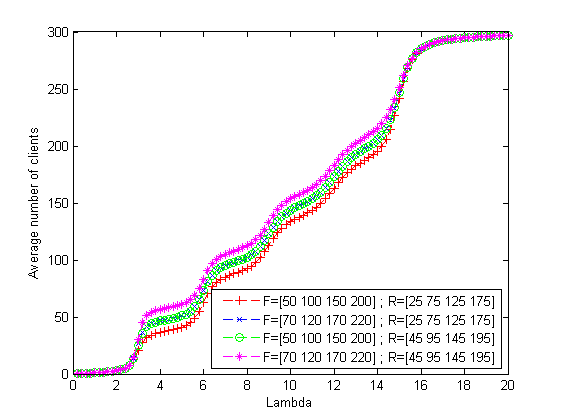
\includegraphics[width=3.5in]{images/test1_fig2}
\caption{Average number of clients in the system versus arrival rate ($\lambda$) : $\mu=1$, $K=5$ and $B=400$}
\label{fig:image-chap4-1_par_1-test1_fig2}
\end{figure}

\begin{figure}[!t]
\centering
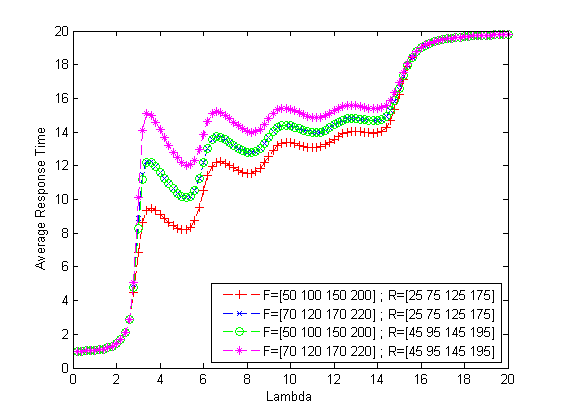
\includegraphics[width=3.5in]{images/test1_fig1}
\caption{Average response time in the system versus arrival rate ($\lambda$) : $\mu=1$, $K=5$ and $B=300$}
\label{fig:image-chap4-1_par_1-test1_fig1}
\end{figure}

\textbf{Experiment 2 :} we analyze the behavior of the average number of servers (VMs) activations per time unit according to arrival rate (figures~\ref{fig:image-chap4-1_par_1_test2_fig1}, ~\ref{fig:image-chap4-1_par_1_test2_fig2} and ~\ref{fig:image-chap4-1_par_1_test2_fig3}). We assume that the number of levels ($K$) $=$ 7, the system capacity ($B$) $=$ 250, $S_{1}=3$ and $S_{i+1}=S_{i}+3$ $\forall i$ (i.e. we activate three VMs when we switch from level $i$ to $i+1$). We vary in X-axis the arrival rate ($\lambda$). We performed tests for different values for thresholds $F$ and $R$. The notation used to write thresholds in figures is $F=[a:b:c]$ (with $a=F_1$, $c=F_{K-1}$ and $\forall i$ $b=F_{i+1}-F_{i}$). In figure~\ref{fig:image-chap4-1_par_1_test2_fig1}, we assume a total overlap between the thresholds of activation $F$ and deactivation $R$ (i.e. $R_1 < F_1 < R_2 < F_2 < R_3 < F_3 < R_4 < F_4 < R_5 < F_5 < R_6 < F_6$). In figure~\ref{fig:image-chap4-1_par_1_test2_fig2} we assume no overlap between activation and deactivation thresholds (i.e. $R_1 < R_2 < R_3 < R_4 < R_5 < R_6 < F_1 < F_2 < F_3 < F_4 < F_5 < F_6$ ). And finally for Figure~\ref{fig:image-chap4-1_par_1_test2_fig3}, we have a partial overlap between the activation and deactivation thresholds (i.e. $R_1 < R_2 < R_3 < F_1 < F_2 < F_3 < R_4 < R_5 < R_6 < F_4 < F_5 < F_6$). 

Results (figures~\ref{fig:image-chap4-1_par_1_test2_fig1}, ~\ref{fig:image-chap4-1_par_1_test2_fig2} and ~\ref{fig:image-chap4-1_par_1_test2_fig3}) show that thresholds values and the difference between activation thresholds and deactivation thresholds influence the shape of the curve of activation rate. We notice that more activation thresholds ($F$) are far from deactivation thresholds ($R$) then less there are activations. Indeed, when thresholds are far from each other, we minimize oscillations between levels, which shows that it is interesting to use a hysteresis models for Cloud resources scaling.

\begin{figure}[!t]
\centering
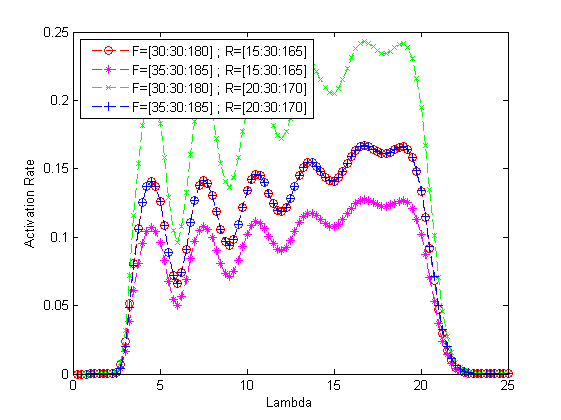
\includegraphics[width=3.5in]{images/test2_fig1}
\caption{Activation rate versus arrival rate ($\lambda$) : $\mu=1$, $K=7$ and $B=250$ (total overlap between activation and deactivation the thresholds)}
\label{fig:image-chap4-1_par_1_test2_fig1}
\end{figure}

\begin{figure}[!t]
\centering
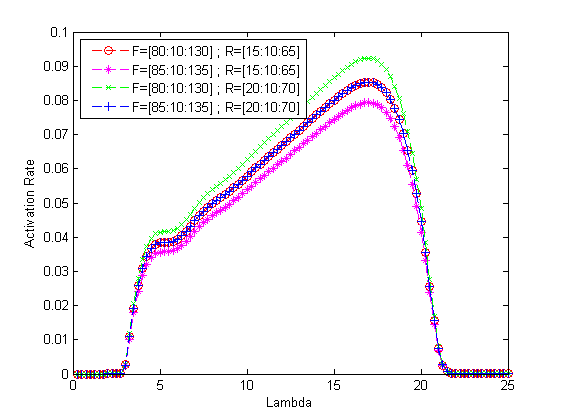
\includegraphics[width=3.5in]{images/test2_fig2}
\caption{Activation rate versus arrival rate ($\lambda$) : $\mu=1$, $K=7$ and $B=250$ (no overlap between activation and deactivation thresholds)}
\label{fig:image-chap4-1_par_1_test2_fig2}
\end{figure}

\begin{figure}[!t]
\centering
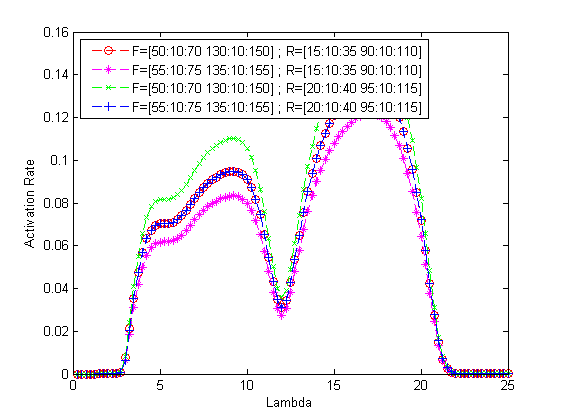
\includegraphics[width=3.5in]{images/test2_fig3}
\caption{Activation rate versus arrival rate ($\lambda$) : $\mu=1$, $K=7$ and $B=250$ (partial overlap between the activation and deactivation thresholds)}
\label{fig:image-chap4-1_par_1_test2_fig3}
\end{figure}


\textbf{Experiment 3 :} we analyze the overall cost (figure~\ref{fig:image-chap4-1_par_1_test3_fig3}). we assume that the arrival rate ($\lambda$) $=$ 4, the number of levels ($K$) $=$ 7 and system capacity ($B$) $=$ 500, $S_{1}=3$ and $S_{i+1}=S_{i}+3$ $\forall i$ (i.e. we activate three VMs when we switch from level $i$ to $i+1$). We set $R=[45\mbox{ }95\mbox{ }145\mbox{ }195\mbox{ }245\mbox{ }295]$ and we vary in X-axis values of $F$. The initial value is $F_{init}=[50\mbox{ }100\mbox{ }150\mbox{ }200\mbox{ }250\mbox{ }300]$ (it corresponds to 0 in the x-axis) then we increase the values of $F$. For example, 10 in the X-axis corresponds to $F$ = $F_{init}+10=[50\mbox{ }100\mbox{ }150\mbox{ }200\mbox{ }250\mbox{ }300]+10$ $=$ [60 110 160 210 260 310]. We measure the overall cost for different values of $C_{A}$ (activationCost in figure~\ref{fig:image-chap4-1_par_1_test3_fig3}). 

We notice that when $F$ increases the overall cost decreases in a first phase then increases after. The reason is that the formula of the overall cost includes both parameters that increases (for example : the average number of clients) and parameters that decreases (for example : the activation rate) according to $F$. The thresholds configuration that ensures the minimal cost depends on $C_{A}$ (activationCost). 

\begin{figure}[!t]
\centering
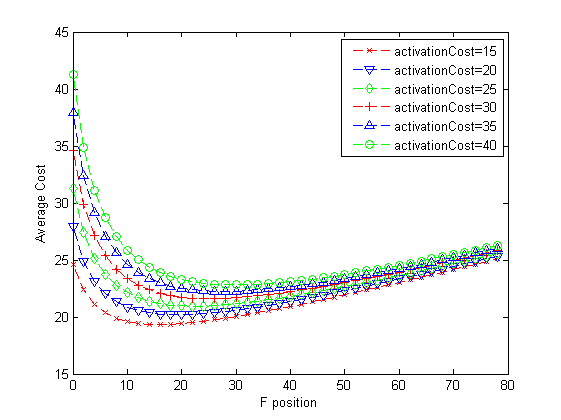
\includegraphics[width=3.5in]{images/test3_fig3}
\caption{Global cost versus $F$ values : $\lambda=4$,  $\mu=1$, $K=7$, $B=500$, $R=[45$ $95$ $145$ $195$ $245$ $295]$ and $F_{init}=[50\mbox{ }100\mbox{ }150\mbox{ }200\mbox{ }250\mbox{ }300]$}
\label{fig:image-chap4-1_par_1_test3_fig3}
\end{figure}

\textbf{Experiment 4 :} we compare a model (\textbf{conf 1}) in which only one VM is activated/deactivated when we switch form one level to another  ($K=32$, $S_1=1$, $S_{i+1}=S_{i}+1$ $\forall i<K$, so $S_{K}=S_{32}=32$) and two models (\textbf{conf2}, \textbf{conf3}) in which many VMs are activated/deactivated when we switch form one level to another ($K=6$, $S_1=1$, $S_{i+1}=2*S_{i}$ $\forall i<K$, so $S_{K}=S_{6}=32$). The overall number of servers (VMs) for the three models is 32 but we have less thresholds in \textbf{conf2} and \textbf{conf3}. In the experiment, we assume that the system capacity ($B$) $=$ 400 and we vary the arrivals rate ($\lambda$). Thresholds of \textbf{conf2} (respectively \textbf{conf3}) were chosen so that the associated model is an upper bound (respectively lower bound) for the performances of the model \textbf{conf1}. Values of F Thresholds are illustrated in figure~\ref{fig:fconfig} and we have $R_{i}=F_{i}-5$ $\forall i$ for all models. 

\begin{figure}[!t]
\centering
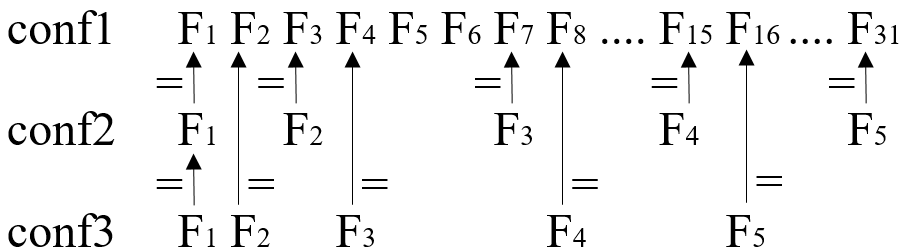
\includegraphics[width=2.5in]{images/F_config}
\caption{The values of F for conf1, conf2 (upper bound) and conf3 (lower bound)}
\label{fig:fconfig}
\end{figure}

Figure~\ref{fig:image-chap4-comp_test1_fig1} illustrates the experiment results (the average number of clients of each model for different arrival rates ($\lambda$)). The result of \textbf{conf2}  (resp. \textbf{conf3}) is always greater (resp. smaller) to the one-by-one model (\textbf{conf1}). \textbf{conf2} and \textbf{conf3} have less thresholds than \textbf{conf1}, so faster to analyse. This idea is useful to analyse large one-by-one models in which we can analyse bounding and smaller models to find a lower and upper bounds for performance rather than analysing the large (so complex) original model. 


\begin{figure}[!h]
  \centering
  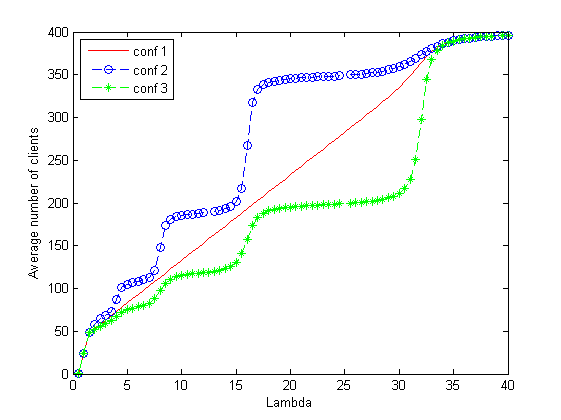
\includegraphics[width=3.5in]{images/comp_test1_fig1}
  \caption{Average response time in the system versus arrival rate ($\lambda$) : $\mu=1$, $B=400$, $32$ servers - Comparison of the three models -}
  \label{fig:image-chap4-comp_test1_fig1}
\end{figure}
% 
% \section{Numerical results}
% We implemented the mathematical methods : (1) aggregation, (2) LDQBD, (3) balance equations, and we performed a set of experiments. In this section, we first present a comparison between the three methods in terms of resolution time. Then we give some numerical examples that aim to show the evolution of performance measures and cost according to arrival rate and thresholds values. All tests were implemented and performed on a machine with "Intel i7" CPU and 8GB of RAM.
% 
% \subsection{Comparison between mathematical methods}
% Table~\ref{tab:Tableau-comparatif-methodes-res} shows the execution time of each mathematical method for different values of : K (the number of levels) and B (the capacity of the system). In the first line we have the smallest instance (K=5, B=300, markov chain with 521 stats), and in the last line we have the largest one (K=1000, B=75000, markov chain with 134921 stats). We observe that the method using the balance equations is the fastest among the three for all instances. Indeed, the calculation is made using formulas that contain basic operations. The aggregation method takes a lot of time for large chains. The reason is the complexity of the GTH approach that we use to resolve the generated sub chains. The method based on the LDQBD structure uses matrix inversion. For $K = 1000$ and $B = 75000$, the program returned an error "out of memory" because of the huge size of the matrix.
% 
% \begin{table}[H]
% %\renewcommand{\arraystretch}{1.3}
% \caption{Comparison between mathematical methods in terms of execution time}
% \label{tab:Tableau-comparatif-methodes-res}
% \centering
% \begin{tabular}{ c | c c c}
%   - & \begin{tabular}{@{}c@{}} Agregation + GTH\end{tabular} & LDQBD & \begin{tabular}{@{}c@{}}Balance equations \end{tabular} \\
%   \hline
%   \begin{tabular}{@{}c@{}}K = 5 \\ B = 300 \\ (521 stats)\end{tabular} & 0.246 sec & 0.017 sec & 0.006 sec \\
%   \hline
%   \begin{tabular}{@{}c@{}}K = 10 \\ B = 750 \\ (1271 stats)\end{tabular} & 1.678 sec & 0.041 sec & 0.011 sec \\
%   \hline
%   \begin{tabular}{@{}c@{}}K = 50 \\ B = 3750 \\ (6671 stats)\end{tabular} & 89.010 sec & 0.496 sec & 0.095 sec \\
%   \hline
%   \begin{tabular}{@{}c@{}}K = 100 \\ B = 7500 \\ (13421 stats)\end{tabular} & 679.342 sec & 2.775 sec & 0.282 sec \\
%   \hline
%   \begin{tabular}{@{}c@{}}K = 500 \\ B = 37500 \\ (67421 stats)\end{tabular} & +30 min & 304.437 sec & 7.408 sec \\
%   \hline
%   \begin{tabular}{@{}c@{}}K = 1000 \\ B = 75000 \\ (134921 stats)\end{tabular} & +30 min & \begin{tabular}{@{}c@{}}"Out of memory"\\ (inversion of \\a very large matrix)\end{tabular} & 34.401 sec \\
% \end{tabular}
% \end{table}
% 
% \subsection{Numerical Examples : Evaluation of performance and cost}
% In this section we consider a threshold-based queuing system with hysteresis and we present some numerical examples that aim observe the evolution of performance measures and cost.
% 
% We first analyze the behavior of the average number of clients in the system (figure~\ref{fig:image-chap4-1_par_1-test1_fig2}) and the average response time (figure~\ref{fig:image-chap4-1_par_1-test1_fig1}). In these figures : the service rate ($\mu$) $=$ 1, the number of servers ($K$) $=$ 5, and system capacity ($B$) $=$ 400. In X-axis, we vary the arrival rate ($\lambda$). Y-axis in figure~\ref{fig:image-chap4-1_par_1-test1_fig2} (resp. figure~\ref{fig:image-chap4-1_par_1-test1_fig1}) represents the average number of clients in the system (resp. the average response time). We performed tests for different values for thresholds $F$ and $R$ (which is represented by the four curves). In figure~\ref{fig:image-chap4-1_par_1-test1_fig2}, the average number of clients increases when the arrival rate ($\lambda$) is bigger. The system is saturated when $\lambda$ reaches $5$. The reason is that above $\lambda=5$, we have $\frac{\lambda}  {K*\mu} >= 1$. If we compare the curves of figure~\ref{fig:image-chap4-1_par_1-test1_fig2} (resp. ~\ref{fig:image-chap4-1_par_1-test1_fig1}), we notice that more the threshold values are significant then more the average number of clients (resp. average response time) is considerable. i.e. when we choose larger thresholds, the servers are activated following a larger number of customers in the system, which results in less performance.
% 
% \begin{figure}[ht]
% \centering
% 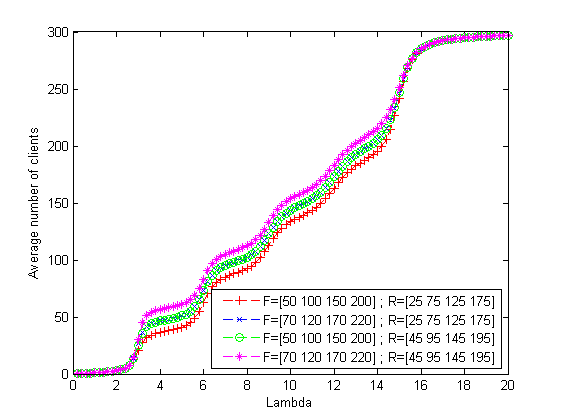
\includegraphics[width=3.5in]{images/test1_fig2}
% \caption{Average number of clients in the system versus arrival rate ($\lambda$) : $\mu=1$, $K=5$ and $B=400$}
% \label{fig:image-chap4-1_par_1-test1_fig2}
% \end{figure}
% 
% \begin{figure}[ht]
% \centering
% 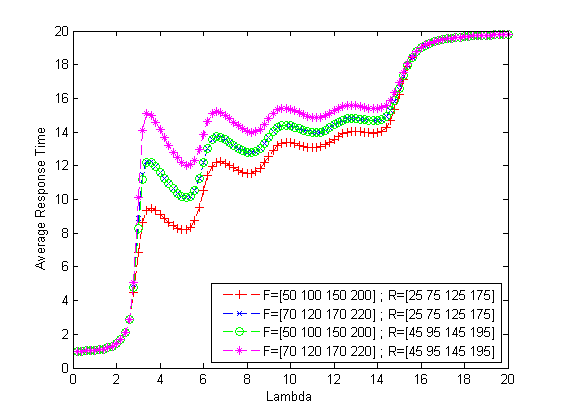
\includegraphics[width=3.5in]{images/test1_fig1}
% \caption{Average response time in the system versus arrival rate ($\lambda$) : $\mu=1$, $K=5$ and $B=400$}
% \label{fig:image-chap4-1_par_1-test1_fig1}
% \end{figure}
% 
% We next analyze the behavior the average number of servers activations per time unit (figures~\ref{fig:image-chap4-1_par_1_test2_fig1}, ~\ref{fig:image-chap4-1_par_1_test2_fig2} and ~\ref{fig:image-chap4-1_par_1_test2_fig3}). In these figures : service rate ($\mu$) $=$ 1, the number of servers ($K$) $=$ 7, and system capacity ($B$) $=$ 250. In X-axis, we vary the arrival rate ($\lambda$).Y-axis represents activation rate (i.e. the average number of servers activations per time unit). We performed tests for different values for thresholds $F$ and $R$. The notation used to write thresholds in the figure is $F=[a:b:c]$ (with $a=F_1$, $c=F_{K-1}$ and $\forall i$ $b=F_{i+1}-F_{i}$). In figure~\ref{fig:image-chap4-1_par_1_test2_fig1}, we have a total overlap between the thresholds of activation $F$ and deactivation $R$ (i.e. $R_1 < F_1 < R_2 < F_2 < R_3 < F_3 < R_4 < F_4 < R_5 < F_5 < R_6 < F_6$). In figure~\ref{fig:image-chap4-1_par_1_test2_fig2} we have no overlap between activation and deactivation thresholds (i.e. $R_1 < R_2 < R_3 < R_4 < R_5 < R_6 < F_1 < F_2 < F_3 < F_4 < F_5 < F_6$ ). And finally for Figure~\ref{fig:image-chap4-1_par_1_test2_fig3}, we have a partial overlap between the activation and deactivation thresholds (i.e. $R_1 < R_2 < R_3 < F_1 < F_2 < F_3 < R_4 < R_5 < R_6 < F_4 < F_5 < F_6$). Results show that thresholds values and the difference between activation thresholds and deactivation thresholds influence the shape of the curve of activation rate. We notice that more activation thresholds ($F$) are far from deactivation thresholds ($R$) then less there are activations. Indeed, when thresholds are far from each other, we minimize oscillations between levels, which shows that it is interesting to use a hysteresis models for Cloud resources scaling.
% 
% \begin{figure}[ht]
% \centering
% 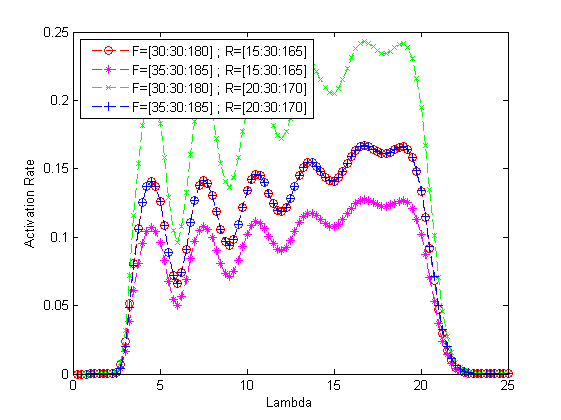
\includegraphics[width=3.5in]{images/test2_fig1}
% \caption{Activation rate versus arrival rate ($\lambda$) : $\mu=1$, $K=7$ and $B=250$ (total overlap between activation and deactivation the thresholds)}
% \label{fig:image-chap4-1_par_1_test2_fig1}
% \end{figure}
% 
% \begin{figure}[ht]
% \centering
% 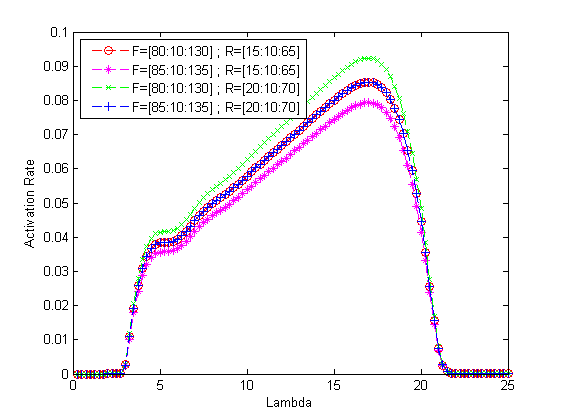
\includegraphics[width=3.5in]{images/test2_fig2}
% \caption{Activation rate versus arrival rate ($\lambda$) : $\mu=1$, $K=7$ and $B=250$ (no overlap between activation and deactivation thresholds)}
% \label{fig:image-chap4-1_par_1_test2_fig2}
% \end{figure}
% 
% \begin{figure}[ht]
% \centering
% 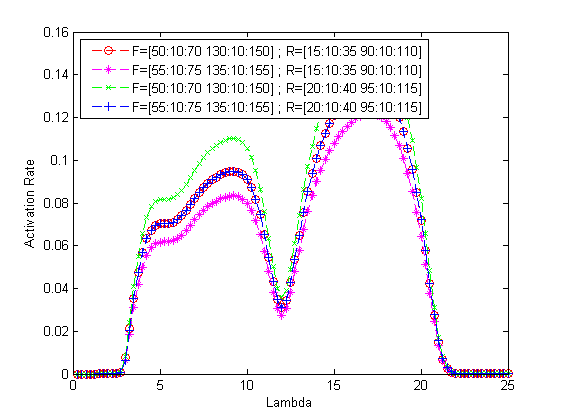
\includegraphics[width=3.5in]{images/test2_fig3}
% \caption{Activation rate versus arrival rate ($\lambda$) : $\mu=1$, $K=7$ and $B=250$ (partial overlap between the activation and deactivation thresholds)}
% \label{fig:image-chap4-1_par_1_test2_fig3}
% \end{figure}
% 
% Finally we analyze the global cost (figure~\ref{fig:image-chap4-1_par_1_test3_fig3}). In this figure : service rate ($\mu$) $=$ 1, arrival rate ($\lambda$) $=$ 4, number of servers ($K$) $=$ 7 and system capacity ($B$) $=$ 500. We set $R=[45\mbox{ }95\mbox{ }145\mbox{ }195\mbox{ }245\mbox{ }295]$ and we vary in X-axis values of $F$. The initial value is $F_{init}=[50\mbox{ }100\mbox{ }150\mbox{ }200\mbox{ }250\mbox{ }300]$ (it corresponds to 0 in the x-axis) then we increase the values of $F$. For example, 10 in the X-axis corresponds to $F$ = $F_{init}+10=[50\mbox{ }100\mbox{ }150\mbox{ }200\mbox{ }250\mbox{ }300]+10$ $=$ [60 110 160 210 260 310]. We measure the global cost for different values of $C_{A}$ (activationCost in the figure). We notice that when $F$ increases the global cost decreases in a first phase then increases after. The reason is that the formula of the global cost includes both the average number of clients that increases and the activation rate that decreases. The thresholds configuration that ensures the minimal cost depends on $C_{A}$ (activationCost).
% 
% \begin{figure}[ht]
% \centering
% 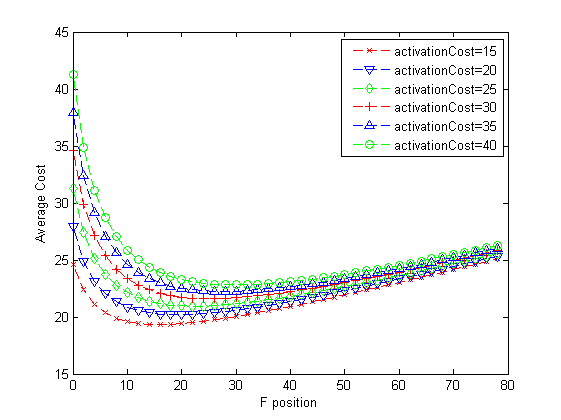
\includegraphics[width=3.5in]{images/test3_fig3}
% \caption{Global cost versus $F$ values : $\lambda=4$,  $\mu=1$, $K=7$, $B=500$, $R=[45$ $95$ $145$ $195$ $245$ $295]$ and $F_{init}=[50\mbox{ }100\mbox{ }150\mbox{ }200\mbox{ }250\mbox{ }300]$}
% \label{fig:image-chap4-1_par_1_test3_fig3}
% \end{figure}

\section{Conclusion}



%Moreover, the bounding models presented in the paper are also interesting and allow to reduce the complexity of the threshold-based queue with hysteresis.





%we observe clearly that when we apply stochastic bounds for batch-arrival distribution, we
%derive also bounds on performance measures and those in relatively less time. And even if a reduction applied on the batch-arrival distribution may seem important (from $500$ states to only $10$ states or $50$ states) the results on performance metrics are, however, very close to the exact results and very accurate. Regarding the computation times, we can remark that for $\rho\simeq 0.2$  we have tended to divide by $9$ the execution time when we reduce the size of the batch-arrival distribution to $bins=50$ and by a little more than $6$ when $\rho\simeq 0.96$, which is quite important given the interesting results obtained.

%We also note that the use of bounding models (Upper bound model and Lower bound model) can also be another way of defining stochastic bounds on performance measurements of the hysteresis model with reduced complexity.



%
%To conclude, through these examples, we show that the results provided after using the stochastic bounds on the batch-arrival distribution, are very accurate and gives a good coverage of the results of the threshold-based queue with hysteresis, and those with considerably reduced computation times.
%Moreover, the bounding models presented in the paper are also interesting and allow to reduce the complexity of the threshold-based queue with hysteresis.
%
%
%



% use section* for acknowledgment
\section*{Acknowledgment}


The authors would like to thank...





% trigger a \newpage just before the given reference
% number - used to balance the columns on the last page
% adjust value as needed - may need to be readjusted if
% the document is modified later
%\IEEEtriggeratref{8}
% The "triggered" command can be changed if desired:
%\IEEEtriggercmd{\enlargethispage{-5in}}

% references section

% can use a bibliography generated by BibTeX as a .bbl file
% BibTeX documentation can be easily obtained at:
% http://mirror.ctan.org/biblio/bibtex/contrib/doc/
% The IEEEtran BibTeX style support page is at:
% http://www.michaelshell.org/tex/ieeetran/bibtex/
\bibliographystyle{IEEEtran}
% argument is your BibTeX string definitions and bibliography database(s)
\bibliography{references}
%


% that's all folks
\end{document}
